\chapter{Selection in protein coding {DNA} sequences}
{
	\hypersetup{linkcolor=GREYDARK}
	\minitoc
}
\label{sec:selection}
Evolutionary trajectory of sequences depends on the forces of mutation, selection and drift, which acts conjointly such that each one of them must be well studied and understood.
However, the previous chapter remained so far elusive on selection, and did not yet question what determines the strength of selection.
More precisely, molecular evolution requires either a given selection coefficient associated to mutation, or that the fitness of each particular sequence to be defined.
In other word, the relationship between sequence and fitness must be elucidated, which is the focus of the present chapter in the special case of protein coding \acrshort{DNA} sequence.
It will seek to clarify the relationship between protein sequence, protein thermodynamic, protein function, and organismal fitness, such as to derive the selective pressures shaping proteins coding \acrshort{DNA} sequences.
It is also important to emphasize whether they are general principles, or do this relationship between sequence and fitness depends on the specific protein, organism, and environment.
To this aims, this chapter will first present the genetic code and classical phylogenetic \glspl{codon} models, which can quantify the strength of selection acting on proteins trough an aggregate parameter (called $\omega$ or $\dnds$).
Application of these phylogenetic models to empirical \acrshort{DNA} alignment provides insight on the variation of selective strength between different orthologous genes, between sites of the same protein, or between branches of the phylogenetic tree.
Subsequently, physico-chemical constrains of proteins and thermodynamics models of protein selection are related to these empirical results.
Finally, given the results on empirical data, generalization of \gls{codon} models into the context of fitness landscapes are presented.

\section{Protein coding {DNA} sequences}

Proteins have a variety of molecular and cellular roles, they are the enzymes that catalyses chemical bonds, they regulate cell processes and control their rates, they carry signals within the cell and across membranes, they bind and transport small molecules, they form cellular structures, and so on.
This variety of roles is accomplished by a variety of three-dimensional shapes.
A protein's three-dimensional shape is in turn determined by the linear one-dimensional sequence of amino-acids, with their size ranging from fewer than $20$ to more than $5000$ amino acids, with an average of about 350 amino-acids.
Just as \acrshort{DNA} is oriented because of the asymetry of nucleotides, proteins are oriented due to asymetry of amino-acids, one end is called \gls{N-ter} and the other end C-terminus, and each amino-acid will interact with the other amino-acids in its spatial vicinity. 

Although each of the 20 different amino acids has unique biochemical properties, they can be classified broadly into four categories determining their solubility and acidity (classification is given in table \ref{table:genetic_code}).
Charged amino-acids can be either basic (positively charged) or acidic (negatively charged).
On the other hand, non charged amino-acids can however be polar due to an uneven charge distribution, such that they can form hydrogen bonds with water.
Consequently, polar amino acids are called hydrophilic, and are often found on the outer surface of folded proteins.
Also, non charged amino-acids can have a uniform charge distribution, and do not form hydrogen bonds with water.
Reciprocally, these non polar amino-acids are called hydrophobic and tend to be found in the core of folded proteins.

\subsection{Genetic code}

Because the $20$ letter alphabet of proteins is different to the $4$ letter alphabet of nucleic acid (DNA and RNA), there is not a one-to-one correspondence between the two alphabets.
Instead, amino acids are encoded by \glspl{codon}, a consecutive sequences of 3 nucleotides, yielding $4^3=64$ possible permutations, more than sufficient to encode the 20 different amino acids.
Moreover, three stop \glspl{codon} signals termination of the protein, such that 61 of the 64 \glspl{codon} are used to encode amino acids.
Since there are 61 coding \glspl{codon} and only 20 amino acids, there is a necessary redundancy in the code.
Thus, amino-acids are encoded by synonymous \glspl{codon}, which are interchangeable in the sense of producing the same amino acid, with the notable exception of methionine and tryptophan.
Altogether, the \acrshort{DNA} genetic code translating \gls{codon} to amino-acids, which is used almost universally by all organisms is given in table \ref{table:genetic_code}.

\begin{table}[H]
	\centering
	\noindent\adjustbox{max width=\textwidth}{%
		\begin{tabular}{|c||l|c|l|c|l|c|l|c||c|}
			\hhline{|-||-|-|-|-|-|-|-|-||-|}
			& \multicolumn{2}{c|}{\textbf{T}} & \multicolumn{2}{c|}{\textbf{C}} & \multicolumn{2}{c|}{\textbf{A}} & \multicolumn{2}{c||}{\textbf{G}} & \\
			\hhline{=#========#=}
			\multirow{4}{*}{\textbf{T}} & TTT & \cellcolor{Nonpolar} & TCT & \cellcolor{Polar} & TAT & \cellcolor{Polar} & TGT & \cellcolor{Polar} & \textbf{T} \\
			\cline{2-2} \cline{4-4} \cline{6-6} \cline{8-8} \cline{10-10}
			& TTC & \cellcolor{Nonpolar} \multirow{-2}{*}{Phenylalanine (Phe/P)} & TCC & \cellcolor{Polar} & TAC & \cellcolor{Polar} \multirow{-2}{*}{Tyrosine (Tyr/Y)} & TGC & \cellcolor{Polar} \multirow{-2}{*}{Cysteine (Cys/C)} & \textbf{C} \\
			\hhline{|~||-|-|-|>{\arrayrulecolor{Polar}}->{\arrayrulecolor{black}}|-|-|-|-||-|}
			& TTA & \cellcolor{Nonpolar} & TCA & \cellcolor{Polar} & TAA & \cellcolor{Stop} Stop (Ochre) & TGA & \cellcolor{Stop} Stop (Opal) & \textbf{A} \\
			\hhline{|~||-|>{\arrayrulecolor{Nonpolar}}->{\arrayrulecolor{black}}|-|>{\arrayrulecolor{Polar}}->{\arrayrulecolor{black}}|-|-|-|-||-|}
			& TTG & \cellcolor{Nonpolar} & TCG & \cellcolor{Polar} \multirow{-4}{*}{Serine (Ser/S)} & TAG & \cellcolor{Stop} Stop (Amber) & TGG & \cellcolor{Nonpolar} Tryptophan (Trp/W) & \textbf{G} \\
			\hhline{|-||-|>{\arrayrulecolor{Nonpolar}}->{\arrayrulecolor{black}}|-|-|-|-|-|-||-|}
			\multirow{4}{*}{\textbf{C}} & CTT & \cellcolor{Nonpolar} & CCT & \cellcolor{Nonpolar} & CAT & \cellcolor{Basic} & CGT & \cellcolor{Basic} & \textbf{T} \\
			\cline{2-2} \cline{4-4} \cline{6-6} \cline{8-8} \cline{10-10}
			& CTC & \cellcolor{Nonpolar} & CCC & \cellcolor{Nonpolar} & CAC & \cellcolor{Basic} \multirow{-2}{*}{Histidine (His/H)} & CGC & \cellcolor{Basic} & \textbf{C} \\
			\hhline{|~||-|>{\arrayrulecolor{Nonpolar}}->{\arrayrulecolor{black}}|-|>{\arrayrulecolor{Nonpolar}}->{\arrayrulecolor{black}}|-|-|-|>{\arrayrulecolor{Basic}}->{\arrayrulecolor{black}}||-|}
			& CTA & \cellcolor{Nonpolar} & CCA & \cellcolor{Nonpolar} & CAA & \cellcolor{Polar} & CGA & \cellcolor{Basic} & \textbf{A} \\
			\cline{2-2} \cline{4-4} \cline{6-6} \cline{8-8} \cline{10-10}
			& CTG & \cellcolor{Nonpolar} \multirow{-6}{*}{Leucine (Leu/L)} & CCG & \cellcolor{Nonpolar} \multirow{-4}{*}{Proline (Pro/P)} & CAG & \cellcolor{Polar} \multirow{-2}{*}{Glutamine (Gln/Q)} & CGG & \cellcolor{Basic} \multirow{-4}{*}{Arginine (Arg/R)} & \textbf{G} \\
			\hhline{|-||-|-|-|-|-|-|-|-||-|}
			\multirow{4}{*}{\textbf{A}} & ATT & \cellcolor{Nonpolar} & ACT & \cellcolor{Polar} & AAT & \cellcolor{Polar} & AGT & \cellcolor{Polar} & \textbf{T} \\
			\cline{2-2} \cline{4-4}\cline{6-6} \cline{8-8} \cline{10-10}
			& ATC & \cellcolor{Nonpolar} & ACC & \cellcolor{Polar} & AAC & \cellcolor{Polar} \multirow{-2}{*}{Asparagine (Asn/N)} & AGC & \cellcolor{Polar} \multirow{-2}{*}{Serine (Ser/S)} & \textbf{C} \\
			\hhline{|~||-|>{\arrayrulecolor{Nonpolar}}->{\arrayrulecolor{black}}|-|>{\arrayrulecolor{Polar}}->{\arrayrulecolor{black}}|-|-|-|-||-|}
			& ATA & \cellcolor{Nonpolar} \multirow{-3}{*}{Isoleucine (Ile/I)} & ACA & \cellcolor{Polar} & AAA & \cellcolor{Basic} & AGA & \cellcolor{Basic} & \textbf{A} \\
			\hhline{|~||-|-|-|>{\arrayrulecolor{Polar}}->{\arrayrulecolor{black}}|-|>{\arrayrulecolor{Basic}}->{\arrayrulecolor{black}}|-|>{\arrayrulecolor{Basic}}->{\arrayrulecolor{black}}||-|}
			& ATG & \cellcolor{Nonpolar} Methionine (Met/M) & ACG & \cellcolor{Polar} \multirow{-4}{*}{Threonine (Thr/T)} & AAG & \cellcolor{Basic} \multirow{-2}{*}{Lysine (Lys/K)} & AGG & \cellcolor{Basic} \multirow{-2}{*}{Arginine (Arg/R)} & \textbf{G} \\
			\hhline{|-||-|-|-|-|-|-|-|-||-|}
			\multirow{4}{*}{\textbf{G}} & GTT & \cellcolor{Nonpolar} & GCT & \cellcolor{Nonpolar} & GAT & \cellcolor{Acidic} & GGT & \cellcolor{Nonpolar} & \textbf{T} \\
			\cline{2-2} \cline{4-4} \cline{6-6} \cline{8-8} \cline{10-10}
			& GTC & \cellcolor{Nonpolar} & GCC & \cellcolor{Nonpolar} & GAC & \cellcolor{Acidic} \multirow{-2}{*}{Aspartic acid (Asp/D)} & GGC & \cellcolor{Nonpolar} & \textbf{C} \\
			\hhline{|~||-|>{\arrayrulecolor{Nonpolar}}->{\arrayrulecolor{black}}|-|>{\arrayrulecolor{Nonpolar}}->{\arrayrulecolor{black}}|-|-|-|>{\arrayrulecolor{Nonpolar}}->{\arrayrulecolor{black}}||-|}
			& GTA & \cellcolor{Nonpolar} & GCA & \cellcolor{Nonpolar} & GAA & \cellcolor{Acidic} & GGA & \cellcolor{Nonpolar} & \textbf{A} \\
			\cline{2-2} \cline{4-4} \cline{6-6} \cline{8-8} \cline{10-10}
			& GTG & \cellcolor{Nonpolar} \multirow{-4}{*}{Valine (Val/V)} & GCG & \cellcolor{Nonpolar} \multirow{-4}{*}{Alanine (Ala/A)} & GAG & \cellcolor{Acidic} \multirow{-2}{*}{Glutamic acid (Glu/E)} & GGG & \cellcolor{Nonpolar} \multirow{-4}{*}{Glycine (Gly/G)} & \textbf{G} \\
			\hhline{|-||-|-|-|-|-|-|-|-||-|}
	\end{tabular}}
	\caption[The Genetic Code]{
		The genetic code \acrshort{DNA} table translating \glspl{codon} into amino-acids.
		Amino-acids are represent into $4$ categories based on the electrochemical properties.
		Non-polar in yellow (\textcolor{Nonpolar}{\ding{110}}), polar in green (\textcolor{Polar}{\ding{110}}), basic in blue (\textcolor{Basic}{\ding{110}}) and finally acidic in red (\textcolor{Acidic}{\ding{110}}).
		Stop \glspl{codon} are represented in black (\textcolor{Stop}{\ding{110}}).
		The synonymous \glspl{codon} encoding for the same amino-acid are usually different by their third \gls{codon} position, the wooble base.
	}
	\label{table:genetic_code}
\end{table}

Biochemical translation from \gls{codon} to amino-acid mechanistically emanates from transfer \acrshort{RNA} (\acrshort{tRNA}).
More precisely, \glspl{codon} binds to \acrshort{tRNA} via an anticodon, three consecutive bases that are complementary and antiparallel to the associated \gls{codon}.
On the other end, \acrshort{tRNA} structure complexes uniquely with one the $20$ amino acid, where the catalytic reaction is performed by aminoacyl-tRNA synthetase \citep{Rich1976}.
As a result, \acrshort{tRNA} genes along with aminoacyl-tRNA synthetase genes constitute the machinery necessary for translating \glspl{codon} into amino-acids .
However, there is not a one-to-one correspondence between the $61$ \glspl{codon} and \acrshort{tRNA} genes.
First, the set of unique sequence of anticodon found in tRNAs genes is actually lower than $61$, and depends on the species but varies from $41$ to $55$ \citep{Goodenbour2006}.
This subset of anticodon sequences necessary to binds all $61$ \glspl{codon} is due to non canonical base pairing\footnote{Canonical base pairing are A-U and G-C, where thymin (T) is replaced by uracil (U) in RNA}.
More precisely, the first two positions in the \gls{codon} bond strongly to the anticodon of the \acrshort{tRNA} (second and third positions), while the third base of the \gls{codon} can be subject to non standard pairing with the first base of the anticodon.
If the anticodon contains a guanine at first position, \glspl{codon} with either U or C at the third position can bounds to this anticodon, and this phenomenon explains why there is not any non-synonymous {transition} from only U to C at third position, and why synonymous \glspl{codon} usually end with T or C.
Also, if the anticodon contains an Inosine at first position, \glspl{codon} with either C, U or A at the third position can bounds to this anticodon, such that for example Leucine encoded by three \gls{codon} (AUU, AUC, AUA) can be bounded by the unique anticodon IAU.
Altogether, non-standard pairing explains why the number of unique anticodons is lower than the number of possible \glspl{codon}, and also explains some part of the structure of the genetic code.

Secondly, \acrshort{tRNA} genes with the same amino-acid binding site and anticodon, which are called isoacceptor \acrshort{tRNA}, may vary in other parts of the \acrshort{tRNA} sequence.
Effectively, many genes can codes for the same isoacceptor \acrshort{tRNA}, where each gene can display varying efficiency and errors in translation, adding a layer of regulation to the process of protein synthesis \citep{Lowe1997,Chan2008,Juhling2008,Lin2019}.
As a result, in some genes some \glspl{codon} are more frequently represented than other possible synonymous \glspl{codon}, an effect named \gls{codon} usage bias.
For genes that are expressed at high levels, the \gls{codon} use is biased in favor of the \glspl{codon} that have an high \acrshort{tRNA} concentration in the cell, ultimately increasing the expression rate and decreasing the rate of mistranslation by reducing the time of occupancy of an open site.
Thus, at a fine-grained molecular scope, a synonymous change can influence mRNA stability, splicing process and protein-folding during translation \citep{Plotkin2011, Rak2018}.
However in the scope of this manuscript, such selection between synonymous \glspl{codon} will not be considered, and selection for proteins will be framed at the amino-acid level in first approximation, and mutation at the nucleotide level.
\begin{table}[H]
	\centering
	\noindent\adjustbox{max width=\textwidth}{%
	\begin{tabu}{|c||c|c|c|c|c|c|c|c|c|c|c|c|c|c|c|c|c|c|c|c|}
		\hline & \textbf{K} & \textbf{N} & \textbf{T} & \textbf{R} & \textbf{S} & \textbf{I} & \textbf{M} & \textbf{Q} & \textbf{H} & \textbf{P} & \textbf{L} & \textbf{E} & \textbf{D} & \textbf{A} & \textbf{G} & \textbf{V} & \textbf{Y} & \textbf{C} & \textbf{W} & \textbf{F}\\
		\hline
		\hline \textbf{K} & - & 4 & 2 & 2 & 0 & 1 & 1 & 2 & 0 & 0 & 0 & 2 & 0 & 0 & 0 & 0 & 0 & 0 & 0 & 0\\
		\hline \textbf{N} & - & - & 2 & 0 & 2 & 2 & 0 & 0 & 2 & 0 & 0 & 0 & 2 & 0 & 0 & 0 & 2 & 0 & 0 & 0\\
		\hline \textbf{T} & - & - & - & 2 & 6 & 3 & 1 & 0 & 0 & 4 & 0 & 0 & 0 & 4 & 0 & 0 & 0 & 0 & 0 & 0\\
		\hline \textbf{R} & - & - & - & - & 6 & 1 & 1 & 2 & 2 & 4 & 4 & 0 & 0 & 0 & 6 & 0 & 0 & 2 & 2 & 0\\
		\hline \textbf{S} & - & - & - & - & - & 2 & 0 & 0 & 0 & 4 & 2 & 0 & 0 & 4 & 2 & 0 & 2 & 4 & 1 & 2\\
		\hline \textbf{I} & - & - & - & - & - & - & 3 & 0 & 0 & 0 & 4 & 0 & 0 & 0 & 0 & 3 & 0 & 0 & 0 & 2\\
		\hline \textbf{M} & - & - & - & - & - & - & - & 0 & 0 & 0 & 2 & 0 & 0 & 0 & 0 & 1 & 0 & 0 & 0 & 0\\
		\hline \textbf{Q} & - & - & - & - & - & - & - & - & 4 & 2 & 2 & 2 & 0 & 0 & 0 & 0 & 0 & 0 & 0 & 0\\
		\hline \textbf{H} & - & - & - & - & - & - & - & - & - & 2 & 2 & 0 & 2 & 0 & 0 & 0 & 2 & 0 & 0 & 0\\
		\hline \textbf{P} & - & - & - & - & - & - & - & - & - & - & 4 & 0 & 0 & 4 & 0 & 0 & 0 & 0 & 0 & 0\\
		\hline \textbf{L} & - & - & - & - & - & - & - & - & - & - & - & 0 & 0 & 0 & 0 & 6 & 0 & 0 & 1 & 6\\
		\hline \textbf{E} & - & - & - & - & - & - & - & - & - & - & - & - & 4 & 2 & 2 & 2 & 0 & 0 & 0 & 0\\
		\hline \textbf{D} & - & - & - & - & - & - & - & - & - & - & - & - & - & 2 & 2 & 2 & 2 & 0 & 0 & 0\\
		\hline \textbf{A} & - & - & - & - & - & - & - & - & - & - & - & - & - & - & 4 & 4 & 0 & 0 & 0 & 0\\
		\hline \textbf{G} & - & - & - & - & - & - & - & - & - & - & - & - & - & - & - & 4 & 0 & 2 & 1 & 0\\
		\hline \textbf{V} & - & - & - & - & - & - & - & - & - & - & - & - & - & - & - & - & 0 & 0 & 0 & 2\\
		\hline \textbf{Y} & - & - & - & - & - & - & - & - & - & - & - & - & - & - & - & - & - & 2 & 0 & 2\\
		\hline \textbf{C} & - & - & - & - & - & - & - & - & - & - & - & - & - & - & - & - & - & - & 2 & 2\\
		\hline \textbf{W} & - & - & - & - & - & - & - & - & - & - & - & - & - & - & - & - & - & - & - & 0\\
		\hline \textbf{F} & - & - & - & - & - & - & - & - & - & - & - & - & - & - & - & - & - & - & - & -\\
		\hline
	\end{tabu}}
\caption[Amino-acids adjacency matrix]{
Number of possible one nucleotide non-synonymous {transitions} between amino-acids, integrating over the underlying \glspl{codon}.
For all the possible $190$ pairs of amino-acids, only $75$ pairs contains at least one non-synonymous {transition}.
}
\label{table:adjacency}
\end{table}
Because mutations are at the nucleotide level and affect only one base, any \gls{codon} can have at most $9$ possible {transitions} to another \glspl{codon} as illustrated in the left panel of figure \ref{fig:graph-codons-aa}.
Moreover, it is possible that some pairs of amino-acids are not accessible through a single non-synonymous {transition} between the underlying \glspl{codon} as illustrated in the right panel of figure \ref{fig:graph-codons-aa}.
In fact, most pairs of amino-acids requires at least two non-synonymous {transitions} ($114$ pairs), in comparison to pairs of amino-acids that are accesible trough a single non-synonymous {transition} ($75$ pairs).

\begin{figure}[htbp!]
	\centering
		\begin{minipage}{0.49\linewidth}
			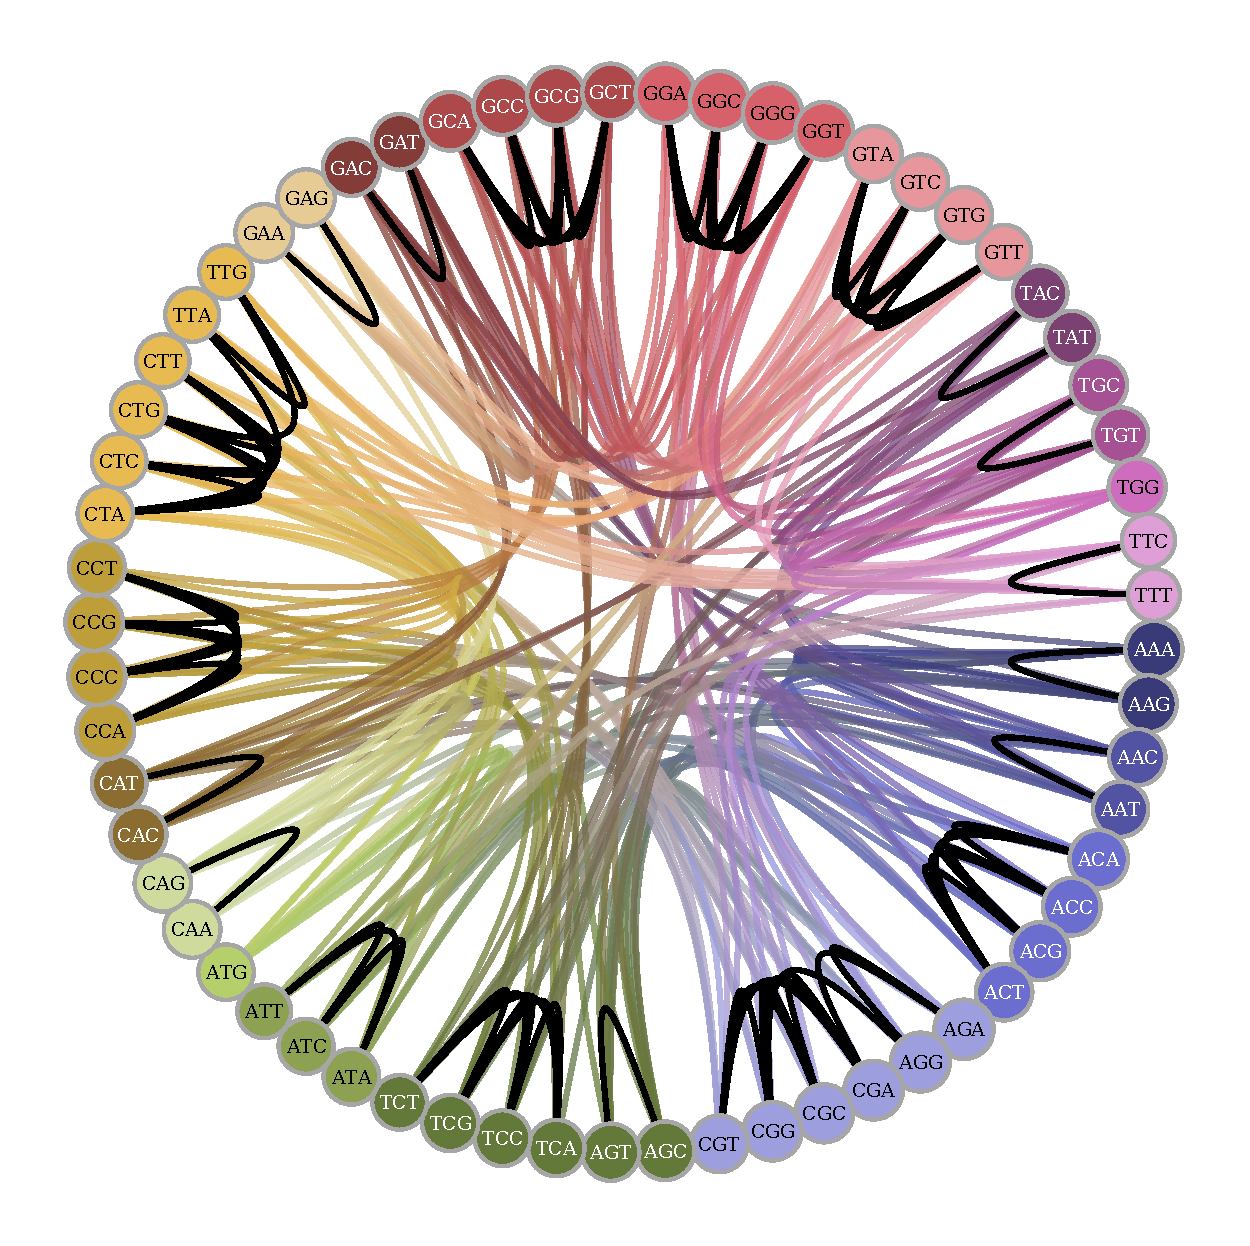
\includegraphics[width=\linewidth, page=1]{figures/gt-codon-tab20b.pdf}
		\end{minipage}%
		\hfill
		\begin{minipage}{0.49\linewidth}
			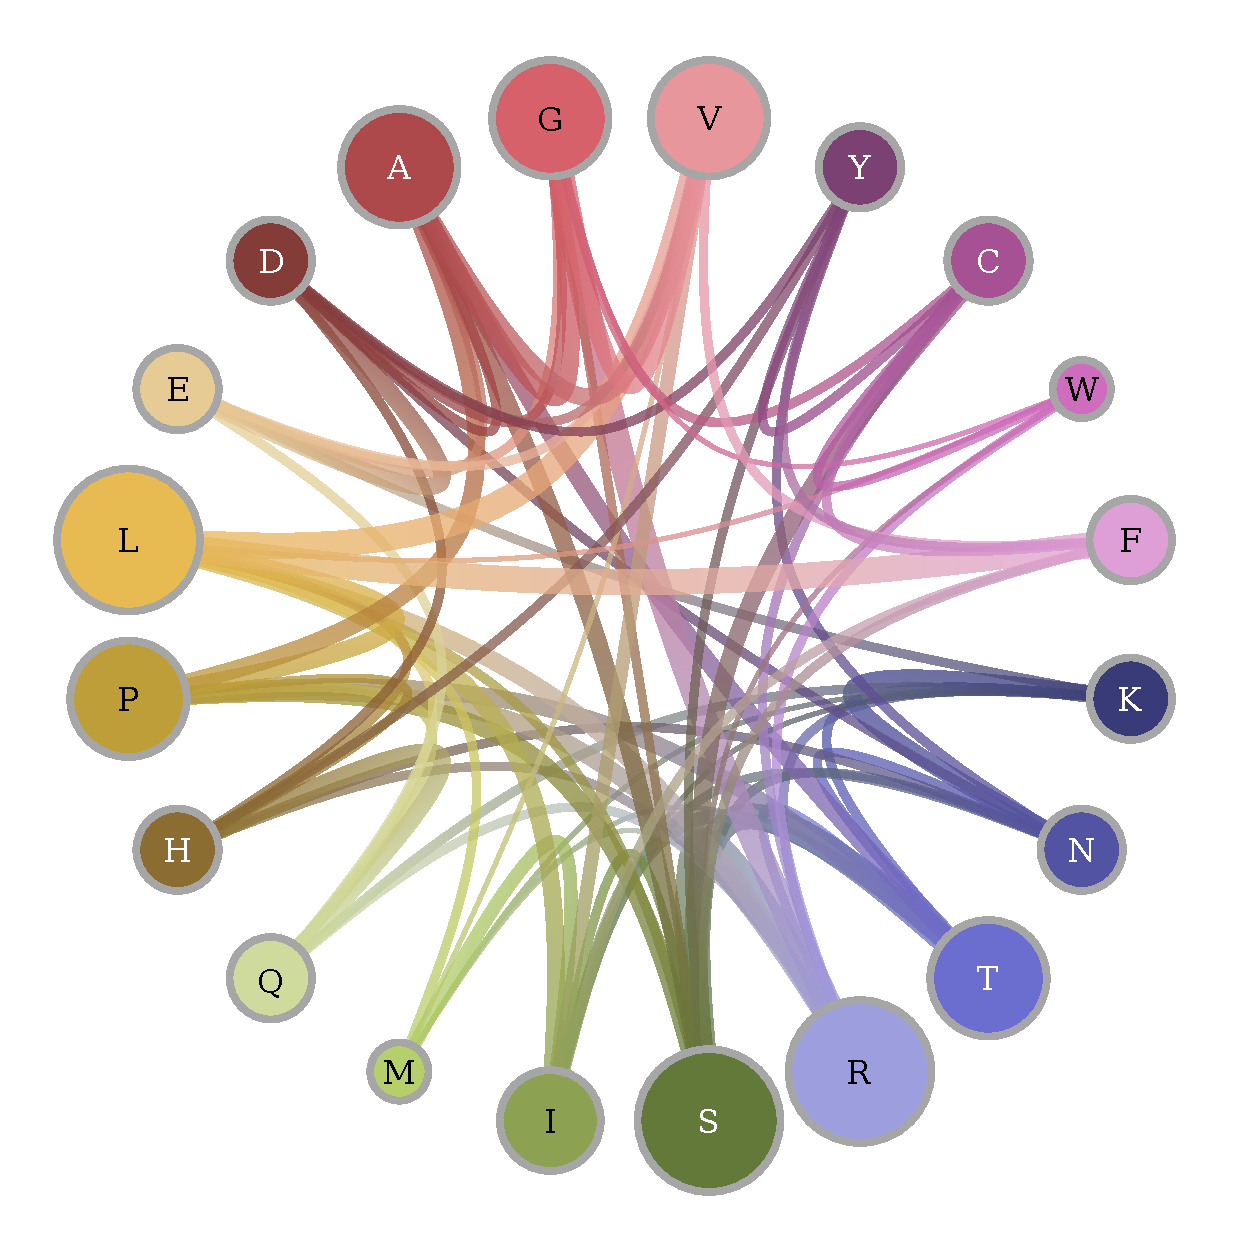
\includegraphics[width=\linewidth, page=1]{figures/gt-aa-tab20b.pdf}
		\end{minipage}

	\caption[Graphs of {codon} and amino-acid transitions]{
		\label{fig:graph-codons-aa}
		Graphs of possible one nucleotide {transition} between \gls{codon} (left panel) and between amino-acid (right panel).
		Nodes corresponds to \glspl{codon} (left panel) and amino-acid (right panel), where their color pictures the encoded amino-acid.
		Additionally, for amino-acids the size of nodes represent the number of underlying \glspl{codon}.
		An edge between two \glspl{codon} depicts a one nucleotide {transition}, such that a \gls{codon} can have at most $9$ possible {transitions}.
		Similarly, an edge between two amino-acids correspond to a one nucleotide non-synonymous {transition} between the underlying \glspl{codon}, and the weight of the edges represent the number of such possible {transitions}.
		Non-synonymous {transition} are represented in colored gradient, while synonymous {transitions} are depicted in black.
		The graph of the $61$ \glspl{codon} contains $263$ {transitions}, $67$ of them are synonymous while $196$ are non-synonymous.
		The radius of the graph is three, such that the most distant amino-acids are at most three {transition} away.
		Codons encoding for the same amino-acid are all fully connected by synonymous changes, expect for Serine where a {transition} for (TCT, TCG, TCC,	TCA) to (AGT, AGC) requires passing through another amino-acid, hence a least two non-synonymous {transitions}.
		From the perspective of amino-acids, the graph of the $20$ amino-acids contains $75$ non-synonymous {transitions}.
		The graph is not fully connected and do not form a clique. Moreover, the graph radius equal to three because a {transition} from Methionine to Tyrosine requires at least three non-synonymous {transitions}.
		Altogether, for all the possible $190$ pairs of amino-acids, $114$ pairs requires at least two non-synonymous {transitions}, and one pair (M-Y) requires at least three non-synonymous {transitions}.
	}
\end{figure}

\subsection{Stability constrains}

The ability of a protein to performs its function depends on the stability of its 3-dimensional folding structure, but also on its ability to bind ligands and interact or no with other protein, both in terms of kinetic and stability.
Altogether, thermodynamics and kinetic of protein are expected to be related to its function, hence to selective constrains \citep{Bastolla2017}.
This section review the main relationship between protein biophysics and selection.

First, a large body of evidence indicates that the stability of globular proteins is a target of natural selection \citep{Sikosek2014}.
The stability of a protein is determined by the Gibbs free energy of its folded states, in comparison to the free energy of the unfolded states.
Similarly to the mutation-selection Markov process defined in the previous chapter, it is possible to derive the equilibrium distribution of states, where fitness is analogous to the opposite of free energy (less energetic state are more stable) and population size to inverse temperature.
As a result, probabilities of observing a specific state, given by Boltzmann equation, is proportional to the exponential of free energy:
\begin{align}
	p(G_F)\propto \e^{- G_F / T}.
\end{align}
In this context, mutations of the proteins stabilizes the protein only if the decrease the free energy of the folded states, more than they decrease the free energy of unfolded states.
For example, a {transition} to an amino-acid that decrease by the same amount the free energy of both folded and unfolded states will have no impact on the stability of the protein.
Theoretically, the stability of a protein can be computed with biophysical of protein, by modeling the atomic structure and the potential energy of contact between residues, computed using Schrodinger's equation and atomic orbitals \textcolor{GREEN}{[References needed]}.
On the other extreme, some models more crudely approximates the structure and dynamic of protein by 2-dimensional lattice models with regular pavement \textcolor{GREEN}{[References needed]}. 
In between these two extremes, many models can approximate with various degrees of liberties and parametrization the relationship from sequence to stability.
Broadly, {transition} from hydrophobic to hydrophilic amino-acids at the surface of protein results in increase stability, and conversely for the protein core.

If the relationship from protein sequence to protein stability is within reach and can be obtained with various degrees of approximations, relationship from stability to fitness is more elusive and difficult to apprehend.
First, it is known the protein stability relates to fitness, as demonstrated by a study of nearly 1000 mutations in beta-lactamase TEM-1 \citep{Jacquier2013}, or illustrated by the use of functional assays to identify stabilizing mutations \citep{Araya2012}.
However, it is not clear whether protein stability increases fitness by being more efficient, or whether it is the deleterious cytotoxic effect of unfolded proteins that result in purifying selection for destabilizing mutations.
Stability-constrained models that take into account negative design for destabilizing misfolded conformations.
At partial answer can be obtained by realizing that \citep{Berezovsky2007, Noivirt-Brik2009, Minning2013} predict that both the \gls{substitution} rate and the entropy are maximal not at exposed sites with few contacts, as observed, but at sites where the number of contacts is intermediate, which can accomodate both hydrophobic and polar amino acids and are predicted to be extremely tolerant to mutations \citep{Jimenez2018}.
On the other hand, when stability with respect to misfolding is not considered, stability-constrained models predict that the variability is maximal at exposed sites with few contacts \citep{Scherrer2012,Echave2015}, but these kinds of models overestimate both the tolerance to mutations and the average hydrophobicity at almost all positions \citep{Jimenez2018} and they score much worse than models that consider misfolding in \gls{likelihood} calculations \citep{Arenas2015a, Arenas2017}, so that models that consider misfolding have to be preferred.
These results support the view that the structural effect of mutations cannot be neglected, in particular at sites with intermediate numbers of contacts that are extremely tolerant to mutations under the point of view of the stability.
Starting from an optimal sequence, mostly destabilizing mutations will occur, but they may reach fixation and accumulate until selection coefficients against new deleterious mutations is too strong, at which point the protein will reach a point of equilibrium called marginal stability \citep{Taverna2002, Bloom2007}.

Importantly, theoretical models also based on protein stability have been invoked to explain this negative correlation between $\dnds$ and expression level \citep{Wilke2006, Drummond2008}, such that selection against protein misfolding induces abundant proteins to evolve to greater stability, where the protein is more constrained and evolve slowly \citep{Serohijos2012}.

Finally, the ability to bind other proteins may interfere with stability against misfolding, and large functional movements may imply a stability cost.
Empirically, residues at functional sites are rarely optimal for stability, so that their mutation is often less destabilizing, while mutations that create new functions tend to be more destabilizing than average \citep{Chi2016}.

\subsection{Aggregation avoidance}

So far, proteins have been seen as independent machinery of the cells, however within the cramped intra-cellular space, proteins are not independent entities but are interactions with the proteome, where protein may either be in free form or engaged in non-specific interactions \citep{Yang2012, Zhang2013}.
In non-specific interactions at the protein surface, stabilizing amino-acids are hydrophilic and destabilizing amino-acids are hydrophobic, sticking to hydrophobic residues in other proteins \citep{Dixit2013,Manhart2015}.
The misinteraction avoidance hypothesis predicts that, compared with lowly expressed proteins, highly expressed proteins disfavour residues that promote misinteraction, exhibit a lower misinteraction probability per molecule and have higher conservation for misinteraction-avoiding residues.

\section{Substitution rate in classical codon models}

Under the approximation that selection occurs for protein, designing \gls{substitution} models at the amino-acid level has the major shortcoming of not taking into account that the underlying mutation process occurs at the nucleotide level.
Conversely, studying evolution of protein coding \acrshort{DNA} sequences only at the nucleotide level, while disregarding the genetic code neglects the consequences that nucleotide variation can have onto protein sequences.
These shortcomings are both addressed by \gls{codon} models, where the complexity of the genetic code is seen as an asset rather than an encumbrance.
Indeed the redundancy in the genetic code can be leveraged to disentangle mutation and selection in protein coding \acrshort{DNA} sequences, under the approximation that selection occurs at the protein level in first approximation, while the mutation process occurs at the \acrshort{DNA} level.
The genetic code allows to split mutations into synonymous and non-synonymous mutations, where synonymous mutations are deemed \gls{neutral}, and non-synonymous mutations are considered under selection \citep{Muse1994,Goldman1994}.

Following the formalism of \gls{codon} models pioneered by \citet{Muse1994}, the $4 \times 4$ mutation matrix $\Mutmatrix$ at the nucleotide level is defined as:
\begin{equation}
\label{eq:mutrates}
\Mutmatrix = \begin{pmatrix}
- & {\mutmatrix_{AC}} & 		{\mutmatrix_{AG}} & 		{\mutmatrix_{AT}} \\
{\mutmatrix_{AC}} & - & {\mutmatrix_{CG}} &		{\mutmatrix_{CT}} \\
{\mutmatrix_{AG}} & 		{\mutmatrix_{CG}} & - & {\mutmatrix_{GT}} \\
{\mutmatrix_{AT}} & 		{\mutmatrix_{CT}} & 		{\mutmatrix_{GT}} & -
\end{pmatrix},
\end{equation}
Grouping nucleotides into \glspl{codon}, mutation rate from \gls{codon} $\ci$ to $\cj$ thus depends on the underlying nucleotide change between the \gls{codon}, if $\ci$ to $\cj$ are only a mutation away, $\nucitoj$ denotes the nucleotide change between the \glspl{codon} and the mutation rate from \gls{codon} $\ci$ to $\cj$ is:
\begin{equation}
\mu_{\itoj} = 
\begin{dcases}
 \mutmatrix_{\nucitoj} \text{ if $\ci$ and $\cj$ are one mutation away,} \\
 0 \text{ else.}
\end{dcases}
\end{equation}

At the \gls{codon} level, synonymous mutations are deemed \gls{neutral} and the rate of \glspl{synonymous} ${\submatrix_{\itoj}}$ is equal to the mutation rate: 
\begin{align}
\submatrix_{\itoj} & = \mu_{\itoj} \\
				  & = \mutmatrix_{\nucitoj}
\end{align}

Conversely, non-synonymous mutations are considered under selection, where their probability of fixation is stretched by a factor $\omega$, and their \gls{substitution} rate is:
\begin{align}
\submatrix_{\itoj} & = \omega \mu_{\itoj} \\
					& = \omega \mutmatrix_{\nucitoj}.
\end{align}
All non-synonymous mutations are considered equivalent, and $\omega$ encompass the average strength of selection exercised on them.
Most importantly, $\omega>1$ is absorbing the signals of an excess in the rate of \glspl{non-synonymous}, indicating that the protein is under adaptive evolution.
Conversely, a default of \glspl{non-synonymous}, leading to $\omega<1$, means the protein is under purifying selection.


Because of this definition, $\omega$ identifies with the rate of \glspl{non-synonymous} over the rate of \glspl{synonymous}, termed $\dnds$.

Throughout this manuscript, the term $\dnds$ will be used to identify the estimation of $\omega$ from protein coding \acrshort{DNA} sequence alignment under the original model of \citet{Muse1994}.
To note, $\omega$ can also be parameterized as function of the average scaled selection coefficient:
\begin{align}
\omega & = \dfrac{S}{1 - \e^{-S}} \text{, where }\\
& \Rightarrow	\begin{dcases}
	S > 0 \iff \omega > 1 \\
	S = 0 \iff \omega = 1 \\
	S < 0 \iff \omega < 1
	\end{dcases}
\end{align}

Altogether, the $61$-by-$61$ \gls{codon} \gls{substitution} matrix of \citet{Muse1994} is defined entirely by the mutation matrix ($\Mutmatrix$), $\omega$ and the genetic code:
\begin{equation}
\begin{dcases}
\submatrix_{\itoj} & = 0 \text{ if $\ci$ and $\cj$ are not one mutation away} \\
\submatrix_{\itoj} & = \mutmatrix_{\nucitoj} \text{ if $\ci$ and $\cj$ are syonymous} \\
\submatrix_{\itoj} & = \omega \mutmatrix_{\nucitoj} \text{ if $\ci$ and $\cj$ are non-syonymous} \\
\submatrix_{\ci, \ci} & = - \sum\limits_{\cj \neq \ci} \submatrix_{\itoj}
\end{dcases}
\label{eq:codon-models}
\end{equation}

It is important to note that under this model, the equilibrium frequencies of all \glspl{codon} are equal, and depends only on the equilibrium frequencies of nucleotides ($\sigma_{A}, \sigma_{C}, \sigma_{G}, \sigma_{T}$):
\begin{align}
\pi_{\ci} & = \dfrac{\sigma_{\ci[1]}\sigma_{\ci[2]}\sigma_{\ci[3]}}{\sum\limits_{\cj}\sigma_{\cj[1]}\sigma_{\cj[2]}\sigma_{\cj[3]} } \\
 & = \dfrac{\sigma_{\ci[1]}\sigma_{\ci[2]}\sigma_{\ci[3]}}{(1 - \sigma_{T}\sigma_{A}\sigma_{A} - \sigma_{T}\sigma_{A}\sigma_{G} - \sigma_{T}\sigma_{G}\sigma_{A} )},
\end{align}
where $\ci[1]$ denotes the nucleotide at position $1$ of \gls{codon} $i$.

Moreover, the relative \gls{substitution} rate at equilibrium $\langle \nu \rangle$ defined by equation \ref{eq:relative-sub-rate}, if restricted to the subset of \glspl{non-synonymous}, identifies to $\omega$:
\begin{align}
\langle \nu \rangle & = \dfrac{ \sum\limits_{\ci} \pi_{\ci} \sum\limits_{\cj \in \NonSyn_{\ci}} Q_{\itoj}}{\sum\limits_{\ci} \pi_{\ci} \sum\limits_{\cj \in \NonSyn_{\ci}} \mu_{\itoj}} \\
					& = \dfrac{ \sum\limits_{\ci} \pi_{\ci} \sum\limits_{\cj \in \NonSyn_{\ci}} \omega \mu_{\itoj}}{\sum\limits_{\ci} \pi_{\ci} \sum\limits_{\cj \in \NonSyn_{\ci}} \mu_{\itoj}} \\
					& = \omega \dfrac{ \sum\limits_{\ci} \pi_{\ci} \sum\limits_{\cj \in \NonSyn_{\ci}} \mu_{\itoj}}{\sum\limits_{\ci} \pi_{\ci} \sum\limits_{\cj \in \NonSyn_{\ci}} \mu_{\itoj}} \\
					& = \omega, 
\end{align}
where $\NonSyn_{\ci}$ is the set of non-synonymous \glspl{codon} neighbors to \gls{codon} $\ci$.
This identity seems so far trivial and unnecessary, but will bear importance later when comparing this phenomenological model to mechanistic models of \gls{codon} \glspl{substitution}.


Models of \gls{codon} \glspl{substitution} can be to applied to protein coding \acrshort{DNA} sequences alignment to estimates the ratio of non-synonymous over \gls{synonymous} rates ($\dnds=\hat{\omega}$).
More precisely, these models can provides estimates of $\dnds$ for the whole gene, for a specific site or for a specific branch of the tree, and whether the sequence evolves under positive or negative selection.
However, in practice, protein are typically under a mix of adaptation and purifying selection, thus typically leading to an $\dnds<1$ even in the presence of positive selection.
Most importantly to the scope of this manuscript, they \gls{codon} models proved to be very valuable to quantify and asses the selective constrains imposed on protein coding sequences.

Importantly, different implementations of phylogenetic \gls{codon} models have been proposed, which parameterize the mutation matrix and the \gls{codon} frequencies in different way \citep{Muse1994, Goldman1994}, ultimately leading to variable fits of the data and different estimation of $\dnds$ on the same dataset. 
However, and fortunately, estimation of $\dnds$ has been proved to be largely insensitive to the underlying \gls{codon} models \citep{Spielman2018}, such that empirical estimation of $\dnds$ using different methods leads to comparable results.

\subsection{Variation across genes}

The increased availability of genomic data together with advancement of computing resources and algorithm prompted an extensive search for the major determining factor of a gene $\dnds$.
Surprisingly, the functional importance of a protein, widely thought to approximate the level of functional constraint, has only a minor role, whereas protein expression level (mRNA concentraion) is found to be a major determinant \citep{Zhang2015}.
Most importantly, this relationship is negative such that genes with high expression level are under stronger purifying selection, or lower $\dnds$ at the level of the gene \citep{Duret2000, Drummond2005a, Zhang2015}.
In unicellular organisms, the mRNA concentration of a gene varies across cell cycle stages and environments, but most studies used data collected from the mid-log phase of growth under rich media, which presumably reflect average concentrations across cell cycle stages.
In multicellular organisms, mRNA concentration data used are typically from the whole organism or are averaged from several examined tissues.
Because of the strong correlation between mRNA and protein concentrations, the negative correlation between protein concentration and evolutionary rate is also strong.

However, even for those proteins of comparable expression levels, their $\dnds$ still span several orders of magnitude \citep{Drummond2008}.
Abundance likewise cannot account for the quasi log-normal distribution of $\dnds$ among genes in a genome, a fact observed from bacteria, yeast, worm, fly, mouse, and humans.
These observations suggest that protein abundance, although a major determinant of $\dnds$, is not its only causal variable.

\subsection{Variation across sites}

Appart from variation across genes, the strength of selection is not typically homogeneous along the protein sequence, and it has been rapidly recognized that the parameter $\dnds$ should not be estimated globally over the entire sequence.
In so-called site-specific phylogenetic \gls{codon} models, $\dnds$ is allowed to vary across sites, either via a finite mixture \citep{Yang2001}, an infinite mixture \citep{Huelsenbeck2006}, or as random effects from a parametric distribution \citep{Lartillot2013}.
Site-specific models had been developed to detect specific site of the sequence under positive recurrent selection \citep{kosiol_patterns_2008}, with a $\dnds>1$, but also proved to be very valuable models to correlate selective pressure and bio-chemical properties os specific sites.

Similarly to search for the determining factors of $\dnds$ at the gene level, extensive search had been conducted at the site level, within a protein.
The major determinant of site-specific $\dnds$ proved to be relative solvent accessibility, where site with higher solvent accessibility display a lower $\dnds$ \citep{Ramsey2011}.
It was later shown that the number of native inter-residue contacts formed by a protein site, which is negatively correlated with the solvent accessibility, is a stronger predictor of site-specific $\dnds$ \citep{Yeh2013}.
Altogether, $\dnds$ changes dramatically between exposed and buried sites in such a way that buried sites tend to evolve more slowly than exposed sites \citep{Echave2016}.
Moreover, this relationship obtained by means of phylogenetic \gls{codon} models can be matched with experiment correlating protein site properties with allelic diversity within population.
In this context, relative solvent accessibility was also found to be a major determinant of adaptive evolution, with most adaptive mutations occurring at the surface of proteins \citep{Moutinho2019}.

The observations that surface residues of globular proteins undergo \gls{substitution} more rapidly than those in the core is generally attributed to the fact that natural selection imposes stronger constraints on buried sites.
It is well known that amino acid residues located inside a protein structure (that is, core residues) have more central roles than surface residues in protein folding stability.

Finally, it is important to keep in mind that selection differs in a way that depends on the specific source and target amino-acid involved in the {transition}.
As a consequence, a single parameter of selection (here $\dnds$) can not disentangle the specific importance of amino-acid chemical properties (polarity, volume, charge, and so on) since all non-synonymous {transitions} are considered equivalent in classical phylogenetic \gls{codon} models \citep{Dutheil2008}.

\subsection{Variation across branches}

Beside variation across genes and site, the strength of selection is not typically homogeneous along the phylogenetic tree, and it has also been recognized that the parameter $\dnds$ should be varying along the tree \citep{Yang1998}.
The motivation was to allow for $\dnds$ to be estimated only on a subset of the phylogeny, based on biological assumption.
For example, such models can detect an adaptive process ongoing during the divergence of one lineage, which can allow for the detection of the proteins responsible for speciation \citep{Yang2001, Zhang2004}.
Moreover, without \gls{prior} knowledge on biological divergence, branches can get clustered together based on their \gls{substitution} rates \citep{Dutheil2012a}.
However, \gls{substitution} rate is a continuous traits, and should evolve smoothly along the phylogeny, such that abrupt shifts are penalized \citep{Huelsenbeck2003,Seo2004}.
I this modeling approach, \gls{substitution} rate of given branch is log-normally distributed around the value of its parent branch, where the standard deviation is proportional to the branch size (in unit of time) \citep{Lartillot2011, Brevet2019}.
In other words, \gls{substitution} rate is seen as a log-Brownian motion along the phylogeny, where the process splits at every node of the tree. 

Similarly to search for the determining factors of $\dnds$ at the gene and site level, environmental variables or life-history traits that can vary between species have been investigated as factor determining $\dnds$ along the phylogeny \citep{Felsenstein1985,Romiguier2014}.
Integrative inference methods combining molecular sequences and lineage specific quantitative traits have also found that $\dnds$ correlates positively with traits such as longevity and body mass \citep{Lartillot2011, Figuet2017}.
Since lineage with a large body size and extended longevity typically correspond to low $\Ne$ \citep{Romiguier2014}, these empirical correlations suggest a negative correlation between $\dnds$ and $\Ne$, thus confirming the theoretical prediction of the \gls{nearly-neutral} theory of evolution.
However, the universality and robustness of the correlation between $\dnds$ and life-history traits is still debated \citep{Nabholz2013, Lanfear2014, Figuet2016}.

Naturally, both these space (site-specific) and time (branch-specific) refinements mentioned above where combined in so called branch-site models \citep{Yang2002, Zhang2004, Pond2011}.
The fine-grained tunning of site-branch models increased statistical power by seeking short and strong episodes of adaptive selection on a background of purifying selection.
However, in the case of Red-Queen processes ongoing on the protein, the episodes detected by branch-site models would merely be a small fraction of the underlying adaptation.
Indeed the overall tree is under adaptive process and one cannot contrast a branch to the rest of the tree.

%The selection coefficient are drawn from a distribution, known as distribution of fitness effects \citep{Welch2008}
%In Wilson, the fitness effect of a mutation is drawn from a fitness distribution that is solely function of $\Ne$, meaning ${P_{\mathrm{fix}}}$ is independent from the current sequence state.
%On the other hand, in the mutation-selection model proposed, the distribution of fitness effects is a function of the current state.
%
%Because its a distribution of fitness effects and not a fitness landscape, features of evolutionary trajectory such as transient positive selection is not represented.
%They are a generic representation of fitness, easily parameterized and inherently taking into account phenomenon such as epistasis.


\section{Mechanistic {codon} models}
In the light of protein biophysics, modeling specific amino-acids physico-chemical properties is a crucial ingredient to represent evolution of protein coding \acrshort{DNA} sequences.
In contrast, classical \gls{codon} models aggregate into a single parameter $\omega$ all amino-acid selective constrains, which specifically be tangential or orthologous depending original and mutated amino-acid.
Classical \gls{codon} model parametrization with a single parameter $\omega$ is equivalent to saying the probability of reaching fixation is the same for any non-synonymous mutation, regardless of the original and mutated amino-acid encoded by the \gls{codon}.
Ultimately, this assumption results in a lack of sensitivity of models seeking deviation from neutrality, since both positive and negative selection are untangled into the same parameter \citep{Rodrigue2008a}.

In contrast, mechanistic models assume that the protein-coding sequence is at mutation-selection balance under a fixed fitness landscape, which is itself characterized by a fitness vector over the $20$ amino-acid at each site \citep{Yang2008, Halpern1998, Rodrigue2010}.
Crucially, the probability of fixation depends on the difference of fitness between the amino-acid encoded by the mutated \gls{codon} ($\fitj$) and the fitness of the amino-acid encoded by the original \gls{codon} ($\fiti$), where $\aai$ denotes the amino-acid encoded by \gls{codon} $i$.
The rate of \gls{substitution} from \gls{codon} $\ci$ to $\cj$ is derived from equation \ref{eq:sub-transion-rates}:
\begin{align}
\submatrix_{\itoj} & = \mu_{\itoj} \dfrac{4 \Ne \left({\fitj - \fiti}\right)}{{1 - \e^{4 \Ne \left({\fiti - \fitj}\right)} }}, \\
& = \mu_{\itoj} \dfrac{\Fitj - \Fiti}{1 - \e^{\Fiti - \Fitj} }.
\end{align}

Altogether, the $61$-by-$61$ \gls{codon} \gls{substitution} matrix of mechanistic \gls{codon} models is defined entirely by the mutation matrix ($\Mutmatrix$), the vector of $20$ amino-acid relative fitness ($\Fit$) and the genetic code:
\begin{equation}
\begin{dcases}
\submatrix_{\itoj} & = 0 \text{ if $\ci$ and $\cj$ are non neighbors} \\
\submatrix_{\itoj} & = \mu_{\itoj} \text{ if $\ci$ and $\cj$ are syonymous} \\
\submatrix_{\itoj} & = \mu_{\itoj} \dfrac{\Fitj - \Fiti}{1 - \e^{\Fiti - \Fitj} } \text{ if $\ci$ and $\cj$ are non-syonymous} \\
\submatrix_{\ci, \ci} & = - \sum\limits_{\cj \neq \ci} \submatrix_{\itoj}
\end{dcases}
\label{eq:propensities-models}
\end{equation}
Moreover, because the process is time-reversible (see previous chapter), from equation \ref{eq:equilibrium-mut-sel}, the stationary distribution equals:
\begin{align}
\pi_{\ci} & = \dfrac{\sigma_{\ci[1]}\sigma_{\ci[2]}\sigma_{\ci[3]}\e^{\Fiti}}{\sum\limits_{\cj}\sigma_{\cj[1]}\sigma_{\cj[2]}\sigma_{\cj[3]}\Fitj }
\end{align}

From a dynamical perspective, a non-synonymous mutation from a \gls{codon} with high fitness to another \gls{codon} will have a low probability of fixation, since the mutated \gls{codon} will have a lower fitness.
At equilibrium this low probability of fixation of the other \gls{codon} result into high frequency of the \gls{codon} with high fitness.
Essentially, at equilibrium the \gls{codon} frequencies only fluctuate at the mutation-selection balance, and all the mutations are \gls{neutral} on average, but slightly deleterious or advantageous, hence the name \gls{nearly-neutral} models \citep{Ohta1973, Ohta1992, Rodrigue2016}.

The specific case of a flat fitness landscape for all amino-acids, with neither a peak nor a valley results in \gls{neutral} evolution where \gls{substitution} rates equal to mutation rates (see equation \ref{eq:sub-equal-mut}).
In contrast, in \gls{nearly-neutral} models, the amino-acids have a fitness landscape fixed in time, but that is not flat with peak and valley.
The difficulty and complexity of \gls{nearly-neutral} models are to estimate the underlying amino-acid fitness landscape \citep{Halpern1998}.

Because of computational complexity, mechanistic models consider multiplicative fitness (additive log-fitness) across sites.
A first approximation of \gls{nearly-neutral} models is that all the positions of the sequence share the same amino-acid preferences.
But it has been rapidly recognized that each site in the \gls{codon} sequence should have its own independent \gls{codon} preferences.
Site-specific amino-acid preferences have been estimated either by maximum \gls{likelihood} \citep{Tamuri2012,Tamuri2014}, by experimental means \citep{Bloom2017}, or in a Bayesian context have been estimated using non-parametric
prior distribution with \gls{Dirichlet-process} \citep{Rodrigue2010, Rodrigue2014}.
Fitting the mutation-selection model on a sequence alignment leads, via equation (\ref{eq:propensities-models}), results to an estimation of the nucleotide mutation rate matrix as well as the fitness landscape of the protein at each site of the sequence.

\subsection{Relationship to classical models}
Mechanistic mutation-selection \gls{codon} models display the important feature of genuinely accounting for purifying selection.
Indeed \citet{Spielman2015} showed mathematically that if the underlying process is \gls{nearly-neutral} \gls{substitution}, the $\dnds$ estimated by the model seeking deviation from neutrality will always be lower than $1$, under the assumption of no \gls{codon} usage bias.
In other word, classical \gls{codon} \gls{substitution} model will interpret a \gls{nearly-neutral} model as purifying selection ($\dnds < 1$).

Indeed, the site-specific predicted rate of non-synonymous over \gls{synonymous} at the mutation-selection balance is obtained as: 
\begin{equation}
\omega_0 = \dfrac{ \sum\limits_{i} \pi_{i} \sum\limits_{j \in \NonSyn_{\ci}} \dfrac{\Fitj - \Fiti}{1 - \e^{\Fiti - \Fitj} }}{\sum\limits_{i} \pi_{i} \sum\limits_{j \in \NonSyn_{\ci} } \mu_{\itoj}},
\end{equation}
where $\NonSyn_{\ci}$ is the set of non-synonymous \glspl{codon} neighbors to \gls{codon} $\ci$.

Even thought classical \gls{codon} models have less parameters than mechanistic \gls{codon} model, it is important to realize they are not nested, such that is impossible to find a given set of parameters for which the two models are equivalent.
They are inherently different, mechanistic models assume a fixed fitness landscape, while classical models assume a fixed selective effect.
The difference is better highlighted in the case of reverse mutations, where a negative selection coefficient of a mutation is always matched by a positive selection coefficient for the reverse mutation in mechanistic \gls{codon} models.
However in classical \gls{codon} models, a negative selection coefficient is matched by an also a negative selection coefficient for the reverse mutation.

Realizing this relationship between classical and mechanistic \gls{codon} models, under the assumption that the protein is under a \gls{nearly-neutral} regime, the predicted $\omega_0$ (mutation-selection model) and the estimated $\dnds$ (classical-model) should be the same \citep{Spielman2015, Spielman2016}.
But assumptions of the models can be broken, resulting in difference between $\omega_0$ and $\dnds$.
Firstly, if amino-acids are under a fluctuating fitness landscape, which is known as a Red-Queen process.
In this case, by definition, the protein sequence is tracking a constantly moving fitness optimum.
Since the protein sequence is always lagging behind the moving target defined by the amino acid preferences, and since \glspl{substitution} are accepted preferentially if they are in the direction of this target, \glspl{substitution} are on average adaptive.
In other word, at the moment of a \gls{substitution} the target amino-acid as a high relative fitness, which can only then decreases trough time.
Thus breaking the assumption of time independence of amino-acid preferences leads to $\dnds \geq \omega_0$.

Secondly, the \gls{nearly-neutral} assumption can also be broken if there is no independence between sites, a phenomenon known as epistasis between sites.
Unfortunately, one consequence of epistatic interactions is that even if a mutation is \gls{nearly-neutral} upon fixation, subsequently fixed mutations on other sites make the original \gls{substitution} more and more deleterious to revert over time \citep{Gong2014, Lunzer2010, Mccandlish2013}.
This effect leads to entrenchment such that instead of lagging behind a moving target, the current amino-acids reinforce its relative fitness.
In other word, at the moment of a \gls{substitution} the target amino-acid has a nearly equal relative fitness, which can only increases with time \citep{Goldstein2016, Goldstein2017}.
Thus, breaking the assumption of independence between sites leads to $\dnds \leq \omega_0$ \citep{Rodrigue2016}.
To summarize, a departure from near-neutrality with a $\dnds \geq \omega_0$ is a signature of an ongoing Red-Queen process and that the protein is under ever changing adaptation.
On the other hand, a $\dnds \leq \omega_0$ is a signature of epistatic interaction between amino-acids.
But one shortcoming of \gls{nearly-neutral} \gls{codon} \gls{substitution} models is that if one does not get a statistical departure from near-neutrality ($\dnds = \omega_0$), it could be due to a mixture of both Red-Queen and epistatic processes that cannot be untied.

\textcolor{GREEN}{[To integrate :
A new parameter-rich structure-aware mechanistic model for amino acid {substitution} during evolution \citep{Chi2018}.
Site-Specific Amino Acid Preferences Are Mostly Conserved in Two Closely Related Protein Homologs \citep{Doud2015}]}

